\documentclass[utf8, 12 pt]{frontiers_suppmat} 
\usepackage{url,hyperref,lineno,microtype}
\usepackage[onehalfspacing]{setspace}

\usepackage{newtxtext,newtxmath}
\usepackage{array}

%\renewcommand\headrulewidth{0 pt}
\newcolumntype{M}{>$ c <$}
\newcolumntype{V}{>$ l <$}

\bibliographystyle{frontiersinSCNS_ENG_HUMS}

\begin{document}
\onecolumn
\firstpage{1}

\title[Supplementary Material]{{\helveticaitalic{Supplementary Material}}}


\maketitle

\begin{Large}
\textbf{A biomechanical approach to infer size-based functional response in aquatic and terrestrial systems}
\end{Large}

\begin{large}
\begin{center}
\textbf{Portalier S.M.J., Cherif M., Fussmann G.F., Loreau M.}
\end{center}
\end{large}

\vspace{2 cm}

\section{Main framework}

Our approach is based on the recently published biomechanical model (Portalier et al., 2019)⁠. This model uses body size and physical features of the medium, to predict predator to prey interactions. \par
Hence, the model requires body masses of both the predator and its prey. The physical parameters are acceleration due to gravity, body density, medium density, and medium viscosity. Then, the model computes all necessary information to predict feasible predator-prey interactions.  \par
In the present article, only elements required for the computation of a functional response will be described. A full description of the model can be found in the original study (Portalier et al., 2019)⁠. A list of parameters computed from the biomechanical model and used in the present study can be found in table S1.\par
Predation implies motion, and motion is constrained by the mechanical properties of the medium. Following the idea developed by Bejan and Marden (2006), motion can be modelled as an oscillatory movement. Animal stroke propels its body upwards and forwards, then the body returns to its original vertical position, but its has moved forward. We decompose motion into two components: a vertical one and a horizontal one. Mechanical factors affect the body in different ways during the whole process (see Fig. S1).

\subsection{Vertical component of motion}
During stroke, the organism applies a thrust force (e.g., muscles, flagella). Part of this force is dedicated to a vertical lift. This upward motion follows Archimedes’ force (due to the difference between medium and body densities), but is opposed to weight (due to gravity) and drag (due to medium density and viscosity). When thrust stops, the body pursues its movement upwards by inertia, until its stops. Then, the body returns to its original vertical position by inertia, following weight, but in opposition to Archimedes' force and drag.

\subsection{Horizontal component of motion}
The other part of the thrust is allocated to the horizontal component of motion. The body is pushed forwards, facing drag. When thrust stops, the body pursues its motion by inertia, until drag stops it. Both vertical and horizontal components are essential: the horizontal component determines the distance travelled between two points, but it requires that the vertical component either lifts the body or the surrounding medium, allowing motion (Bejan and Marden, 2006).

\subsection{Animal speed}
Using this framework, the model can compute animal speed. The maximal muscular output that an organism can developed is related to its size (Marden  Allen, 2002). Then, the model computes the energetic cost associated to a given motion sequence according to the initial thrust force developed in the vertical ($F_{Mv}$) and horizontal planes ($F_{Mh}$), and the distance covered during the active phase in the vertical ($x_v$) and horizontal planes ($x_h$). 

\begin{equation}
	Work= \int _{t_0} ^{t_{force}} F_{Mv} x_v \; \mathrm{d}x + \int _{t_0} ^{t_{force}} F_{Mh} x_h \; \mathrm{d}x
\end{equation}
The work can then be divided by the total duration of the sequence (from $t_0$ to $t_3$) to yield a cost \textit{per time} ($Cost_{pt}$).
\begin{equation}
	Cost_{pt}=\frac{Work}{t_3} 
\end{equation}
The model can then compute a species-specific speed ($\overline{v}$) that leads to a maximal speed to a minimal cost.
\begin{equation}
	(F_{Mv},F_{Mh}) \Rightarrow \text{Min} \left( \frac{Work}{\overline{v}} \right)	
\end{equation}
The computed species-specific speed fits existing data remarkably well (Fig. 1 main text).

\section{Predation}
Predation is broken up into three successive sequences: a predator needs to search, capture and then handle its prey. Each predation sequence leads to time expenditures. Thus, predation on a given prey requires time for searching ($t_s$), time for capturing ($t_c$) and time for handling ($t_h$) this prey. Each predatory activity implies motion, and motion is constrained by physical factors (mentioned above). \par
%\begin{equation}
%tt
%\end{equation}
\vspace{0.5 cm}
\subsection{Search sequence}
During searching time, both predator and prey move at a species-specific speed ($v_p$ for predator and $v_n$ for prey) that scales with body size. A given predator will encounter an individual from the prey population at a rate $E_r$ (Rothschild and Osborn, 1988)⁠ depending on prey abundance ($N$), and predator detection distance ($D_P$). Predator detection distance scales with its size (Pawar et al., 2012).
\begin{equation}\label{encountercomplete}
	E_r= \frac{\pi D_P^2 (v_N^2+3v_P^2)}{3v_P} N	
\end{equation}
For a given predator and a given prey, all parameters are constant except prey abundance ($N$). Thus, encounter rate (Eq. \ref{encountercomplete}) can write 
\begin{equation}\label{encounter}
	E_r= \beta N	
\end{equation}

\subsection{Capture sequence}
Once a prey is detected, the capture sequence begins. The predator jumps and tries to seize its prey, while the prey tries to escape, the distance between the predator and the prey is assumed to be the detection distance of the prey (that scales with prey size). Relative speed at time when predator reaches the prey leads to a capture probability ($P_C$) using a logistic function.
\begin{equation}
	P_c=\frac{1}{1+\frac{v_N}{v_P}}
\end{equation}
If the predator cannot reach the prey, then $P_C = 0$. 

\subsection{Handling sequence}
Last, the predator is kept busy during the time needed to consume the prey: the handling time ($t_h$).
\begin{equation}
	t_h=t_{cons}+t_{dig}
\end{equation}
where $t_{cons}$ is consumption time, and $t_{dig}$ is digestion time. 
\begin{equation}
	t_{cons}=B_t \frac{ M_N}{B_s} 
\end{equation}
where $B_t$ is bite time, $B_s$ is bite size, $M_N$ is prey mass. Bite size scales with predator size (Wilson and Kerley, 2003).
\begin{equation}
	B_s=\rho _b  \frac{4}{3} \pi \left( \frac{B_0}{2} \left( \frac{M_P}{M_{0b}} \right)^{0.32} \right)^3	
\end{equation}
where $B_0$ is bite diameter at reference size, $M_p$ is predator mass, $M_{Ob}$ is reference size, and $\rho _b$ is body density. Bite time depends on bite size (Laca et al., 1994)⁠. 
\begin{equation}
	B_t=0.1 B_s^2
\end{equation}
Digestion time writes (Hendriks, 1999)
\begin{equation}
	t_{dig}=t_{dig0}  \frac{M_P}{B_s}  M_N^{0.25}
\end{equation}
where $t_{dig0}$ is digestion time for 1 kg of organism. \par

\subsection{Time computation}
Overall, the biomechanical model gives the total time that a predator needs to feed on a prey (for searching, capturing and handling the prey). Searching time is assumed to be the inverse of encounter rate times the probability of capture (i.e., the time needed to contact one prey that would lead to a successful capture).
\begin{equation}\label{search}
	t_s= \frac{1}{E_r P_c}
\end{equation}
Capture time ($t_c$) is the time needed for the predator to reach the prey during that jump. Last, handling time ($t_h$) is the time needed to consume and digest the prey. \par

\subsection{Functional response}
The functional response is defined as the inverse of the time needed for searching, capturing and handling one unit of prey. 
\begin{equation}\label{nativefunction}
	f(N)= \frac{1}{t_s+t_c+t_h}
\end{equation}
Using equations (Eq. \ref{encounter}) and (Eq. \ref{search}) to replace search time, equation (Eq. \ref{nativefunction}) writes
\begin{equation}
	f(N)= \frac{1}{\frac{1}{E_r P_c}+t_c+t_h}=\frac{1}{\frac{1}{N \beta P_c}+t_c+t_h}
\end{equation}
And rearranging
\begin{equation}
	f(N)=\frac{N \beta P_c}{1+N \beta P_c (t_c+t_h)}
\end{equation}
Under this form, one can recognize a modified version of Holling’s disk equation (Holling, 1961)⁠, where $\beta P_c$ represents attack rate, and where capture and handling times are taken into account instead of handling time only.
\par
Given the assumptions made on the encounter rate (Eq. \ref{encountercomplete}), it is a type II functional response. In addition to prey abundance ($N$), its value changes according to both predator size, prey size and the medium (i.e., aquatic versus terrestrial).
\par

\subsection{Predicted attack rate and handling time according to body size}
The model predicts attack rate and handling time according to predator and prey body masses. It allows investigating the overall trends for these parameters across a wide range of sizes. It appears that attack rate mostly varies with predator size (i.e., a larger predator attacks prey more efficiently). For a given predator, attack rate slightly decreases with increasing prey size (Fig. S2A). Predator size is bounded for very small predators since they do not move fast enough to contact and/or capture any prey. There is an upper prey size limit for all predators: due to the model assumptions, a predator cannot capture a prey larger than itself. 
\par
Handling and capture times mostly vary with prey size (a larger prey requires more time to be reached and consumed). But a larger predator will be capture and consume a given prey faster than a smaller predator (Fig S2B). There is an upper prey size limit and a lower predator size limit for similar reasons as attack rate.    
\par  

%\bibliography{test}

\clearpage
\begin{table}[ht]
\begin{center}
\doublespacing
\caption{List of symbols used throughout the article}
\begin{tabular}{MlMV}
	\multicolumn{1}{c}{Symbol}&\multicolumn{1}{c}{Meaning}&\multicolumn{1}{c}{Value}&\multicolumn{1}{c}{Unit} \\ \hline
	f(N) & Functional response & & \text{ind.s}^-1 \\
	N & Prey abundance &  & \text{ind.m}^{-3} \\
	t_s & Search time & & \text{s} \\
	t_c & Capture time &  & \text{s} \\
	t_h & Handling time & & \text{s} \\
	t_{cons} & Consumption time & & \text{s} \\
	t_{dig} & Digestion time & & \text{s} \\
	E_r & Encounter rate & & \text{ind.s}^{-1} \\
	D_P & Predator detection distance & & \text{m} \\
	v_n & Prey speed & & \text{m.s}^{-1} \\
	v_p & Predator speed & & \text{m.s}^{-1} \\
	P_c & Capture probability & & \text{dimensionless} \\
	B_s & Bite size & & \text{kg} \\
	B_t & Bite time & & \text{s} \\
	M_P & Predator size & & \text{kg} \\
	M_N & Prey size & & \text{kg} \\
	B_0 & Bite diameter at reference size & 0.26 & \text{mm} \\
	M_{0b} & Reference size for bite diameter & 2.9 & \text{kg} \\
	\rho _b & Body density & 1080 & \text{kg.m}^{-3} \\
	t_{dig0} & Reference digestion time & 2.3*10^4 & \text{s.kg}^{-1} \\
\end{tabular}
\end{center}
\end{table}

\clearpage
\begin{figure}[ht]
\begin{center}
\doublespacing
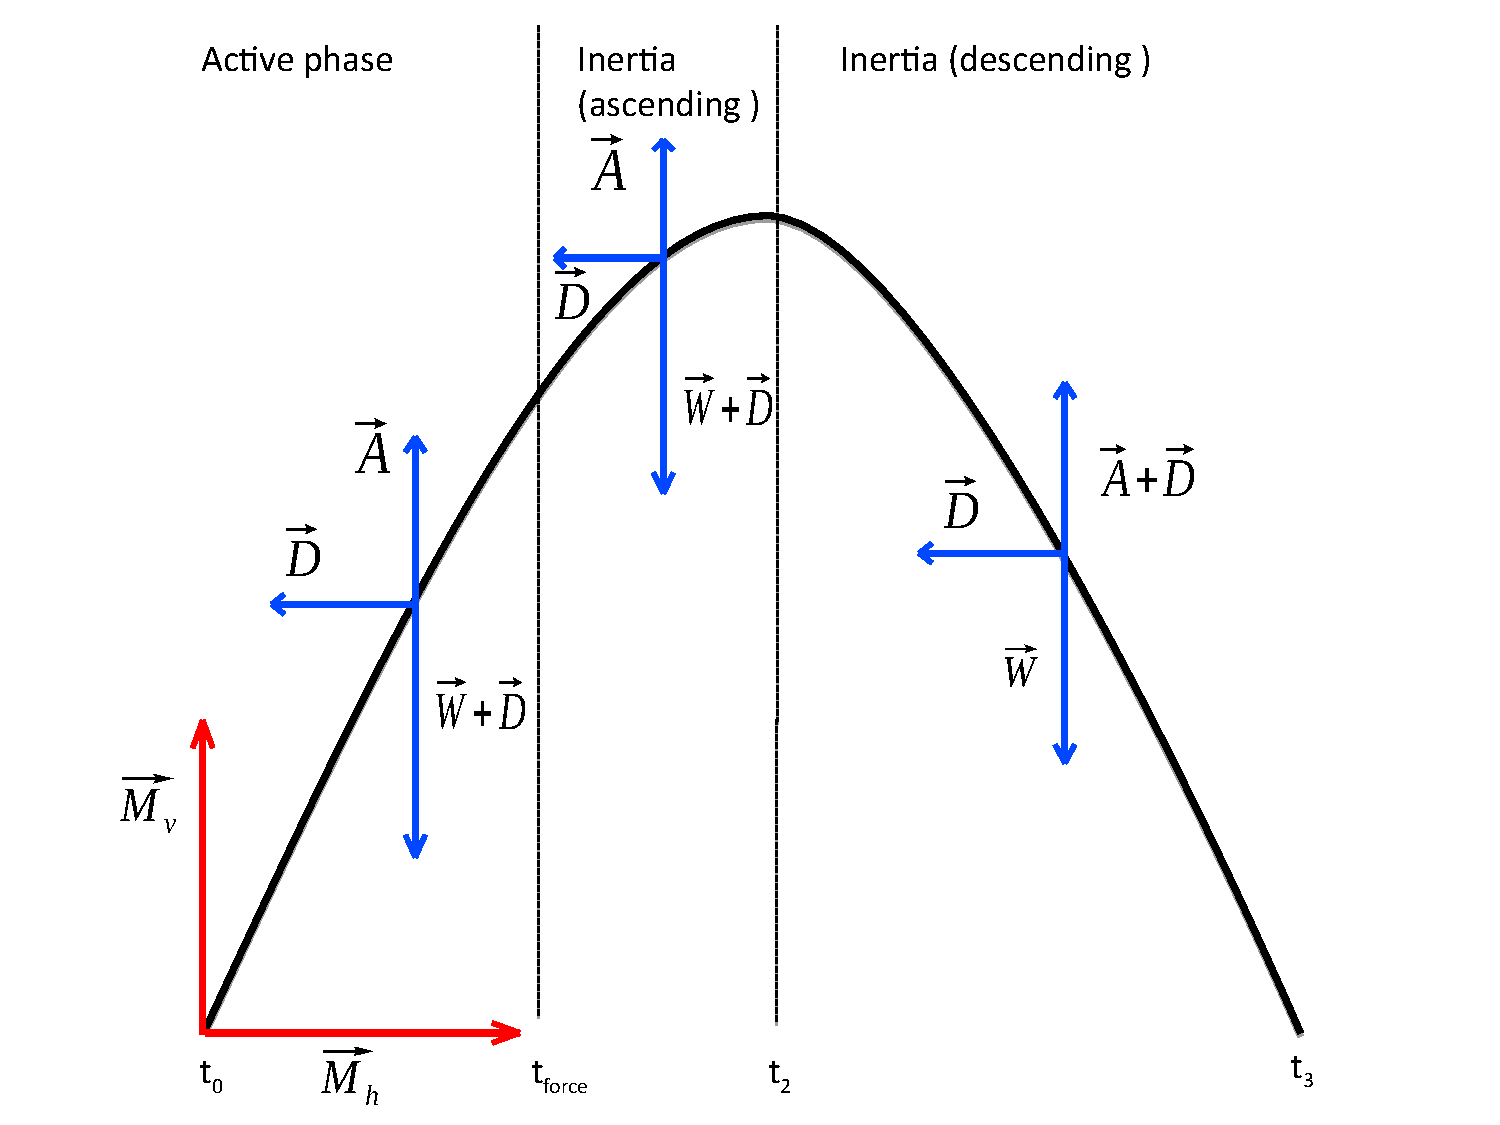
\includegraphics[width = 18 cm, keepaspectratio]{Figure_Forces}
\caption{Framework for the computation of animal motion, represented as an oscillation. Red arrows represent thrust force due to animal stroke, and split between a vertical ($M_v$) and a horizontal component ($M_h$). Blue arrows represent forces due to mechanical factors of the medium. The sequence is decomposed into three phases. During the active phase, thrust force is applied. The body moves upwards, facing weight ($W$) and drag ($D$), but following Archimedes’ force ($A$) and forwards, facing drag, then stroke ends, the body pursue its motion by inertia. Then, the body returns to its original vertical position (descending) by inertia facing Archimedes’ force and drag, but following weight.}
\end{center}
\end{figure}

\clearpage
\begin{figure}[ht]
\begin{center}
\doublespacing
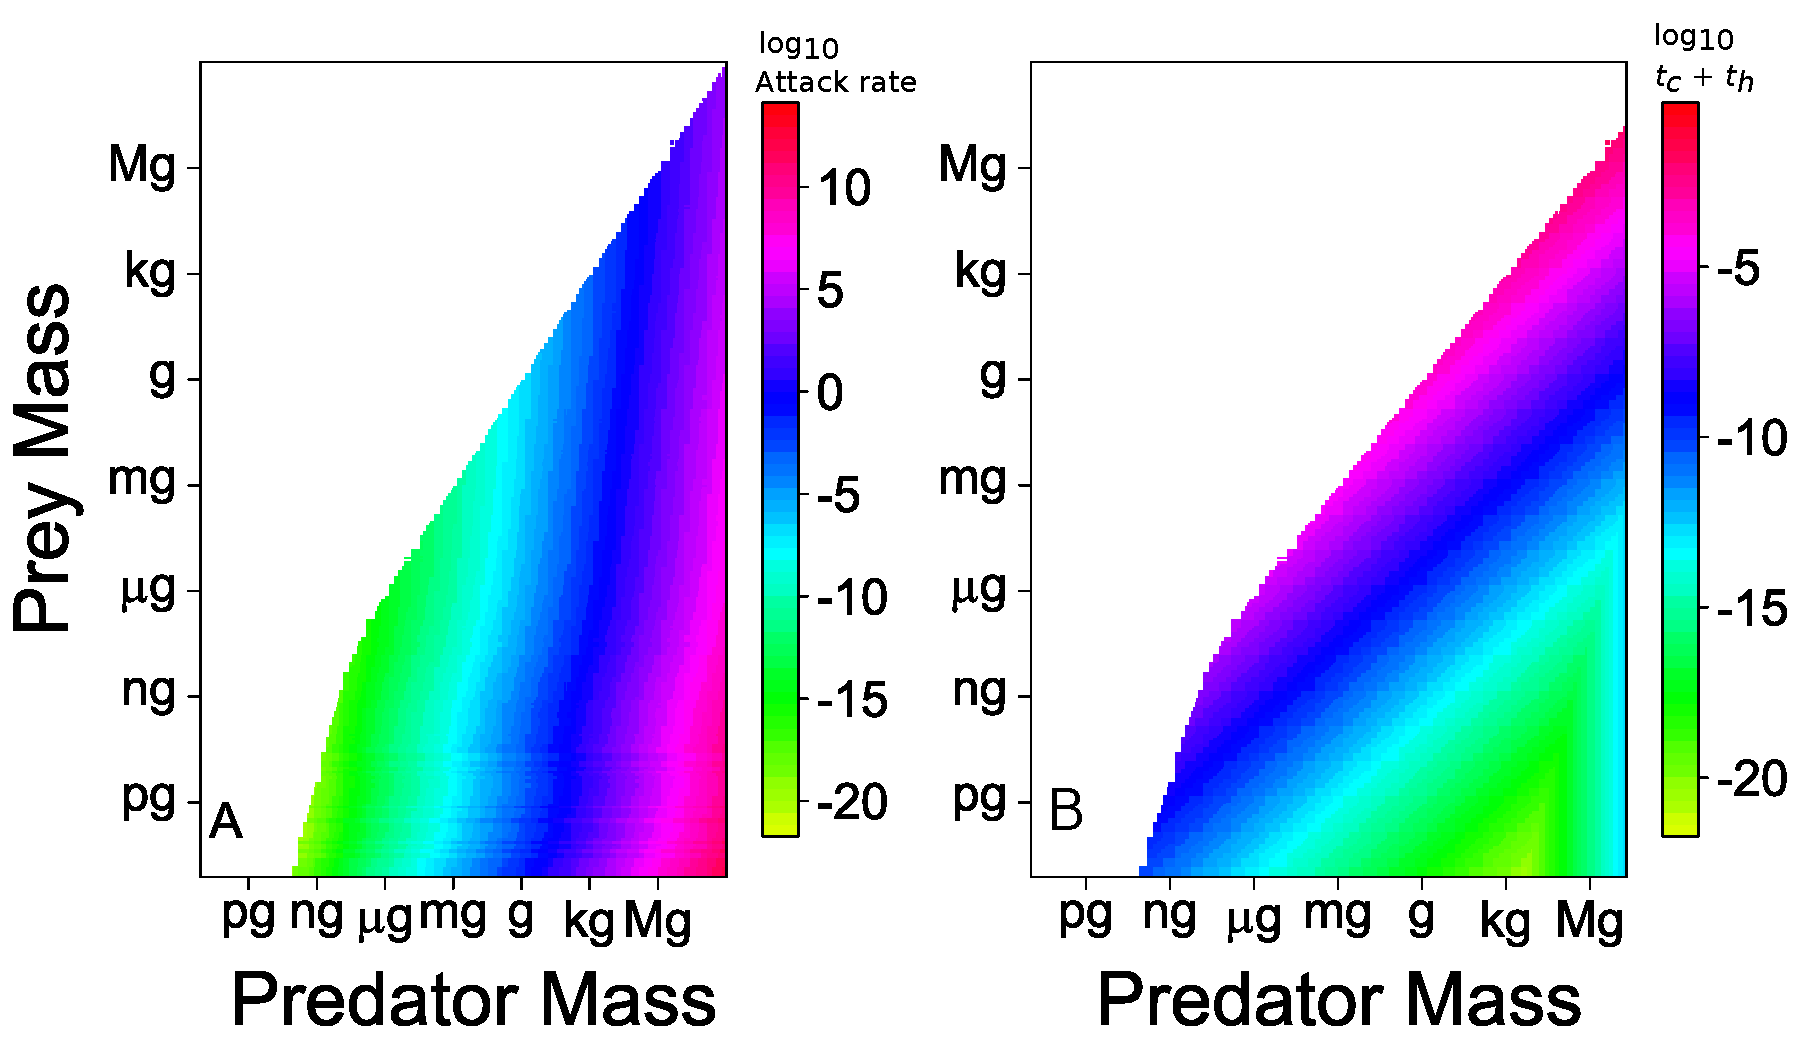
\includegraphics[width = 18 cm, keepaspectratio]{Attack_Rate_Map2}
\caption{Predicted attack rate (A) and capture + handling times (B) according to predator and prey sizes. The white area represents cases where a predator is unable to find, capture or handle the prey, which means that the interaction is not feasible. There is a lower predator size that occurs when the predator do not move fast enough to contact and/or capture any prey. The upper prey size occurs when the predator is unable to capture the prey (due to model assumptions). Attack rate mostly varies with predator size. Capture and handling times mostly vary with prey size for a given predator.}
\end{center}
\end{figure}
\end{document}
